\section{Calculating Bin Sizes}

\begin{figure}[!htb]
\caption{Entropy comparison between bin sizes}
\label{bins}
    \centering
    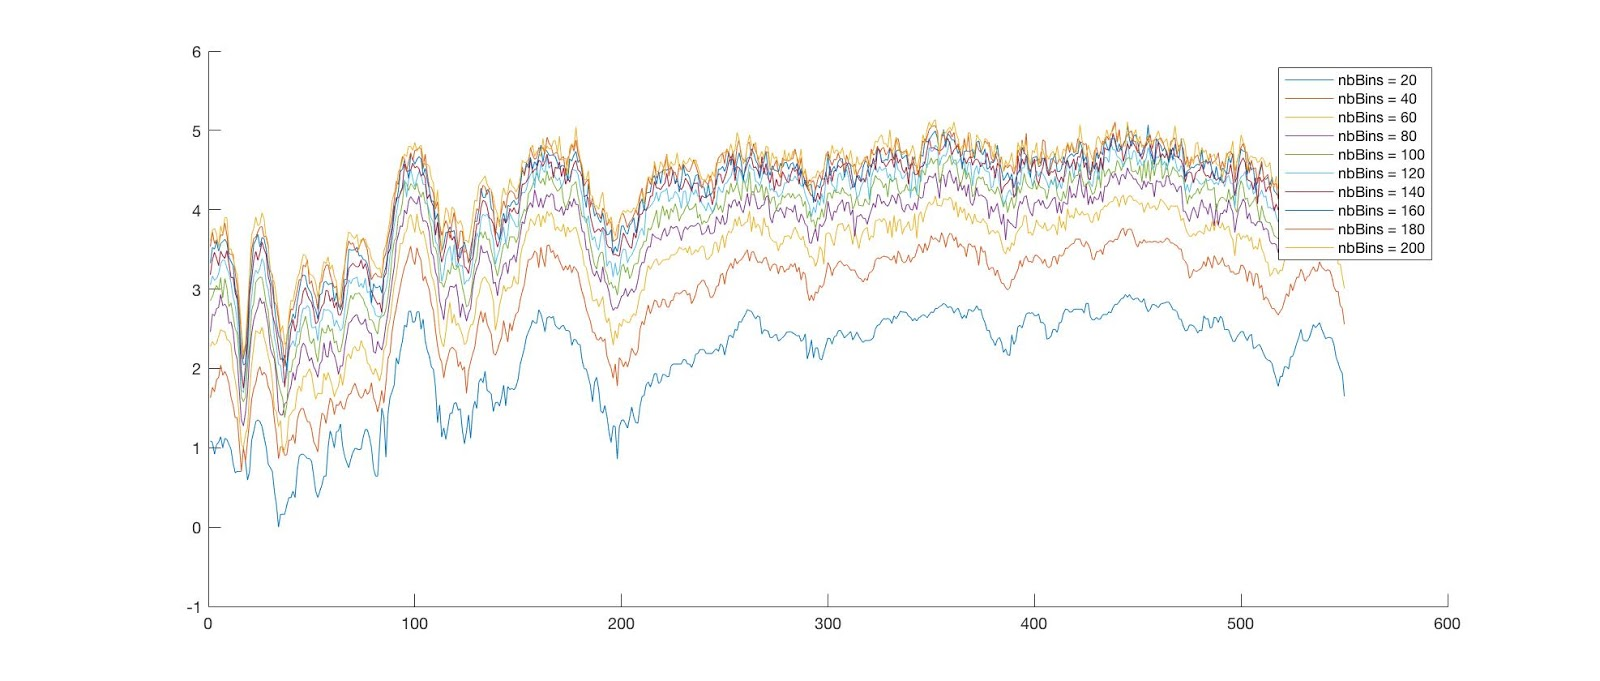
\includegraphics[width=1.2\textwidth]{fig/bins}
\end{figure}

\section{Comparing Common Regions}

\begin{figure}[!htb]
\caption{Experiment}
\label{all-channel-1}
    \centering
    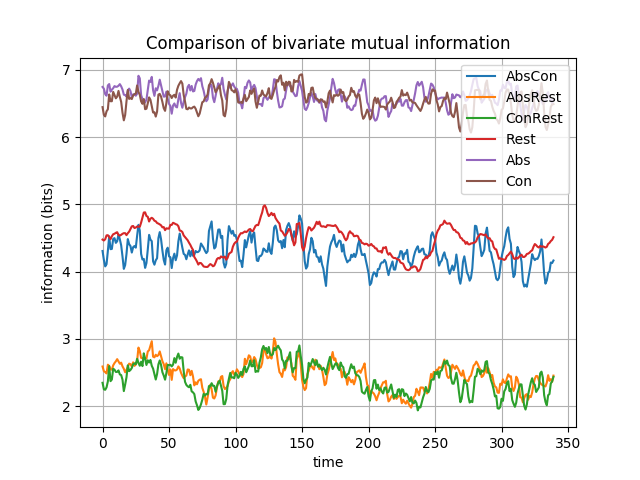
\includegraphics[width=\textwidth]{fig/all-channel-1}
\end{figure}

\begin{figure}[!htb]
\caption{Comparison}
\label{comp-1}
    \centering
    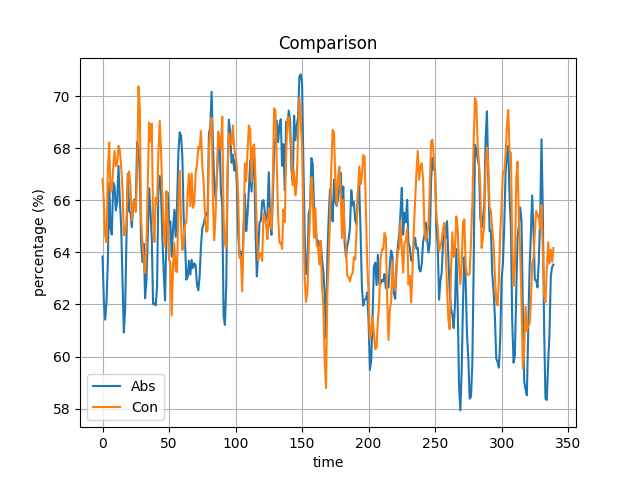
\includegraphics[width=\textwidth]{fig/comp-1}
\end{figure}

\section{Per Subject Comparison}
\subsection{Effect of Trials Used}

\begin{figure}[!htb]
\caption{Entropy comparison between bin sizes}
\label{10-trials}
    \centering
    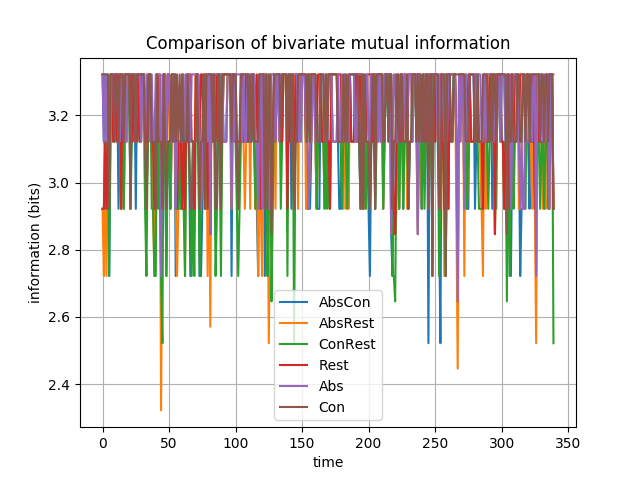
\includegraphics[width=\textwidth]{fig/subject1_10trials_all-channel-1}
\end{figure}

\begin{figure}[!htb]
\caption{Entropy comparison between bin sizes}
\label{40-trials}
    \centering
    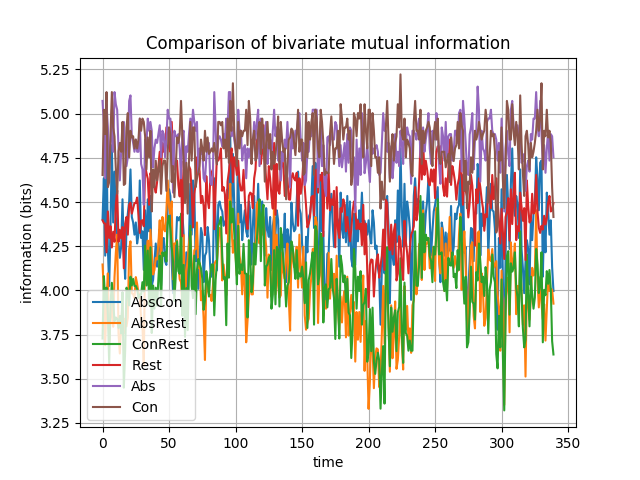
\includegraphics[width=\textwidth]{fig/subject1_40trials_all-channel-1}
\end{figure}

\begin{figure}[!htb]
\caption{Entropy comparison between bin sizes}
\label{all-trials}
    \centering
    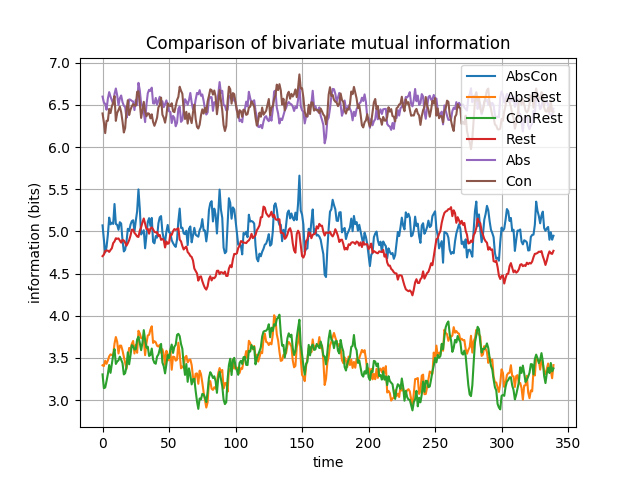
\includegraphics[width=\textwidth]{fig/subject1_alltrials_all-channel-1}
\end{figure}